% Copyright (C) 2018 by latexstudio <http://www.latexstudio.net>
%
% This program is free software: you can redistribute it and/or modify
% it under the terms of the GNU General Public License as published by
% the Free Software Foundation, either version 3 of the License, or
% (at your option) any later version.
%
% This program is distributed in the hope that it will be useful,
% but WITHOUT ANY WARRANTY; without even the implied warranty of
% MERCHANTABILITY or FITNESS FOR A PARTICULAR PURPOSE.  See the
% GNU General Public License for more details.
%
% You should have received a copy of the GNU General Public License
% along with this program.  If not, see <http://www.gnu.org/licenses/>.
%

\section{参考文献篇}
%
%
%\begin{faq}{参考文献中的特殊字符或字母}
%\end{faq}
%
%
%\begin{faq}{BibTeX
%  不理解的作者列表}
%
%BibTeX 只支持三种姓名格式: * First von Last * von Last, First * von
%Last, Jr, First
%
%多个姓名之间必须使用``and''连接,如
%
%\begin{verbatim}
%author = {Knuth, Donald E. and Lamport, Leslie},
%\end{verbatim}
%\end{faq}
%
%
%\begin{faq}{BibTeX
%  排序和名字前缀}
%\end{faq}
%
%
%\begin{faq}{BibTeX
%  中的大写字母}
%
%英文标题中常使用的大小写方式有:
%
%\begin{enumerate}
%  \def\labelenumi{\arabic{enumi}.}
%  
%  \item
%  Title case:
%  句首字母大写,并且除冠词、连词和短介词以外的词首字母大写,这里说的``短''介词一般指不超过
%  4 个字母的介词。比如``The Quick Brown Fox Jumps over the Lazy Dog'';
%  \item
%  Sentence case:
%  句首字母和一些专有名词的首字母大写,同普通的英文句子大小写方式一样,如``The
%  quick brown fox jumps over the lazy dog''。
%\end{enumerate}
%
%BibTeX 根据 bst 样式文件可以将题名保留原大小写,或转为 sentence
%case。所以用户在 bib 数据库中著录标题的正确方式是,统一使用 title
%case,并将需要专有名词用大括号括起来。
%
%\begin{verbatim}
%title = {Finite Element Methods for {Maxwell's} Equations},
%\end{verbatim}
%
%注意尽量避免将一个词中个别字母用大括号括起来,如``\{M\}axwell's'',这可能会导致字母的间距有问题,建议将整个词括起来,如``\{Maxwell's\}''。
%\end{faq}
%
%
%\begin{faq}{如何选择参考文献的风格}
%
%参考文献的风格一般是期刊或会议模板指定 bst
%的,作者应仔细阅读投稿要求和模板使用说明,根据规定使用合适的
%bst。通常有以下方式:
%
%\begin{enumerate}
%  \def\labelenumi{\arabic{enumi}.}
%  
%  \item
%  在文档中声明 \verb|\bibliographystyle{ieeetran}|
%  \item
%  在模板的文档类选项中使用合适的参数,如 \verb|\documentclass[authoryear]{ustcthesis}|。
%\end{enumerate}
%\end{faq}
%
%
%\begin{faq}{BibTeX
%  参考文献数据库}
%
%BibTeX 的 bib 文件是一个记录已阅文献的数据库,但是通常不建议手动编译 bib
%文件,建议:
%
%\begin{enumerate}
%  \def\labelenumi{\arabic{enumi}.}
%  
%  \item
%  使用 JabRef 或 Zotero 等文献管理工具导出 bib 文件创
%  \item
%  使用 \href{https://scholar.google.com/}{Google Scholar} 或
%  \href{https://cn.bing.com/academic}{Bing 学术}导出 bib 条目建
%\end{enumerate}
%\end{faq}
%
%
%\begin{faq}{创建参考文献风格}
%
%BibTeX 的风格文件 bst
%是使用一种后缀语言写的代码,如果对编程能力比较自信的话,可以阅读 BibTeX
%的文档 btxdoc 和 btxhak,btxbst.doc 文件提供了标准 bst
%风格的代码注释,另外还可以阅读 ttb 和 The LaTeX Companion 等资料。
%
%如果不习惯 bst 的编程语言,可以使用 custom-bib 工具,在命令行下运行latex
%makebst,回答一系列问题生成自己的bst。
%
%另外还可以考虑使用 biblatex,它提供更方便的接口用于自定义参考文献格式。
%\end{faq}
%
%
%\begin{faq}{参考文献中的数字格式}
%
%参考文献表中的数字格式是由 @biblabel
%控制的,可以通过重定义该命令来修改格式。比如将数字修改为左对齐:
%
%\begin{verbatim}
%\makeatletter
%\renewcommand\@biblabel[1]{[#1]\hfill}
%\makeatother
%\end{verbatim}
%\end{faq}
%
%
%\begin{faq}{BibTeX文献条目列表}
%
%科技论文通常要求参考文献表中的文献必须在正文中引用,但是在某些特殊情况下仅需要列出
%bib 数据库中的文献,可以使用 \nocite{*}
%命令列出调用的bib中所有条目,或者使用类似\nocite{ref1,ref2,ref3}命令列出需要显示的条目。
%\end{faq}
%
%
%\begin{faq}{制作参考文献的HTML}
%\end{faq}
%
%
%\begin{faq}{BibTeX中的多字母缩写}
%\end{faq}
%
%
%\begin{faq}{多个参考文献表}
%
%natbib宏包与Donald Arseneau和Niel
%Kempson编写的chapterbib宏包兼容,该宏包允许在一个文档内有多个独立的参考文献列表。通常用法是一本书的各章有独立的参考文献列表,尤其是在各章由不同作者独立编写时。
%\end{faq}
%
%
%\begin{faq}{同一位置多文献引用}
%
%只需要将多篇文献的bibkey用英文半角逗号分隔写在一个cite指令的选项里即可。如:
%
%\begin{verbatim}
%\cite{knuth84,lamport86}
%\end{verbatim}
%\end{faq}
%
%
%\begin{faq}{非英文参考文献条目}
%
%什么叫非英文参考文献条目?是指bibkey么?一般不建议用中文,处理好编码格式,无殊。
%中文的参考文献条目,与英文条目并没有什么差别,只是注意编码。目前处理中文推荐用xelatex
%编译 utf8 编码的文件。因此中文的 bib 条目也应该用 utf8 编码。
%\end{faq}
%
%
%\begin{faq}{BibTeX
%  文献手写很困难,有没有什么工具能够生成?**}
%
%多数时候,我们无需自己手写 BibTeX 文献条目。从
%\url{https://scholar.google.com/}、\url{https://academic.microsoft.com/}、
%\url{https://cn.bing.com/academic?mkt=zh-CN}
%或者期刊、数据库的网站上都能够导出 BibTeX 文献条目。 老牌的文献管理软件
%EndNote 也支持生成 BibTeX 格式的数据库,详情见
%官网\url{https://endnote.com/}。 开源软件 JabRef 甚至支持 BibTeX
%文献条目的导入、导出和管理,详情见 官网\url{http://www.jabref.org/}。
%Zetero 使用起来也非常方便,详情见官网 \url{https://www.zotero.org/}。
%谷歌学术、知网、百度学术、万方数据库等在线数据库也是可以支持导出 .bib
%文件的,至于哪家的数据条目更全,就得你自己去甄别了。
%\end{faq}
%
%
%\begin{faq}{如何使用 BibTeX
%  排版参考文献}
%
%\begin{itemize}
%  
%  \item
%  准备一份 BibTeX 数据库,假设数据库文件名为 books.bib,和 LaTeX
%  源代码一般位于同一个目录下。
%  \item
%  在源代码中添加必要的命令,如
%  
%  \bibliographystyle{abbrv}
%  
%  ,
%  
%  \bibliography{books}
%  
%  。假设源代码名为 demo.tex。其中,
%  
%  \cs{bibliographystyle}
%  
%  设定参考文献的格式。\textbackslash{}bibliography
%  告诉系统使用哪个数据库和参考文献列在哪个位置。
%  \item
%  写好了以上两个文件之后,我们就可以开始编译了。例如在命令行中执行以下命令
%\end{itemize}
%
%\begin{verbatim}
%xelatex demo
%bibtex demo
%xelatex demo
%xelatex demo
%\end{verbatim}
%
%或者选择一个可以自动检测是否有参考文献的编辑器,如果有,它会自动执行以上四个命令,但是有时候会遇到检测不到的情况,这时你只需要清理一下辅助文件即可。
%\end{faq}
%
%
%\begin{faq}{如何将参考文献条目录入到正文中}
%
%理工科类论文很少用。
%\end{faq}
%
%
%\begin{faq}{bib文件的重建}
%
%用文本编辑器如Notepad++, Sublime
%Text或WinEdt或专门文献管理软件JabRef,BibDesk等创建文件,改名为 ref.bib
%文件,往里头添加参考文献目录。参考如下:
%% \includegraphics{https://images-cdn.shimo.im/VKQ8uAycksg1zPlo/image.png!thumbnail}
%在.bib文件中,可以采用 TeXStudio 提供的参考文献格式,在自行修改内容
%% \includegraphics{https://images-cdn.shimo.im/0OgCsRQoufMTDJ75/1.png!thumbnail}
%上面的类型有两种选择 BibTeX 和 BibLaTeX ,后者的选择更为广泛。
%参考文献一般不自己书写,而是有可以直接导入。 一般直接 Google
%学术搜索出来的文献或者引用知网,如下:
%% 
%%\includegraphics{https://images-cdn.shimo.im/L1fAEZmW9tYDVTYT/VRI1FEC62J_C6_QSK_P0_0.png!thumbnail}
%点击上图红圈的引号-\textgreater{}
%% \includegraphics{https://images-cdn.shimo.im/N8tFzuXsCM8rOPjF/image.png!thumbnail}
%在点击最左侧的 BibTeX -\textgreater{}
%% \includegraphics{https://images-cdn.shimo.im/81Z6BGei8ycQf1uK/image.png!thumbnail}
%将其复制黏贴到你的 ref.bib 文件中即可。
%在知网上的文献查询需要下载安装如下软件:
%% \includegraphics{https://images-cdn.shimo.im/ZsikCVGdjGIKBqSN/image.png!thumbnail}
%两个都装好了之后,该软件需要自行注册登陆使用。
%然后打开知网,会看到如下:
%% \includegraphics{https://images-cdn.shimo.im/DVEoaSyHJKwmbSjH/2.png!thumbnail}
%右上角红圈圈到的就是为浏览器安装的 Zotero Connector插件,在此需要打开
%Zotero
%软件,点击之后显示下图,选择需要的文献。
%% \includegraphics{https://images-cdn.shimo.im/w4eu1WOehS05gJ0g/image.png!thumbnail}
%然后 Zotero 软件如下显示
%% \includegraphics{https://images-cdn.shimo.im/VFUjYs5MvKQz522e/image.png!thumbnail}
%然后文件-\textgreater{}导出文献库-\textgreater{}导出格式 BibTeX
%确定保存生成的bib文件,可以将这个 bib 文件中的参考文献全部复制黏贴到你的
%ref.bib
%文件中,也可以单独作为一个新的bib文件,在正文区则需要添加多个bib文件就可以,用命令
%\begin{verbatim}
%\bibliography{test,ref}
%\end{verbatim}
%
%,多个bib文件用逗号分隔即可。同时为引用的参考文献需要命令 \nocite{*}
%来将未引用的文件全部排版出来。 注:百度学术、万方数据库等也支持导出 .bib
%文件。
%\end{faq}
%
%
%\begin{faq}{如何减少参考文献条目行间距}
%
%文献条目间距为 \cs{itemsep},默认值4.5pt plus 2pt minus
%1pt,可通过指令 \verb|\addtolength{\itemsep}{距离}| 调整。
%\end{faq}
%
%
%\begin{faq}{按照章节分开参考文献条目}
%
%可看看chapterbib宏包。 \#\# 引文的排序及压缩
%
%这个取决于使用的宏包,常用的natbib宏包可以使用sort或者sort\&compress选项激活相应的排序或排序并压缩功能。
%\#\# 引文列表排序
%
%这个取决于bst,一般模板都有指定的bst。 \#\# BibTeX中过长的字符串 \#\#
%按照``unsrt''规则的目录重排序 \#\# BibTeX参考文献中的URL
%
%调用url或者xurl宏包即可正常使用url,也可以看看href宏包。 \#\# 基于Plain
%TeX的BibTeX的使用 \#\# 常用的biblatex参考文献样式
%
%biblatex除了可以应用自带的标准样式外,还可以使用其他作者提供的第三方样式,这里介绍一些常用的样式:
%* 国外常用 * APA * MLA * 国内 * GB7714-2015
%样式名\textbar{}用法\textbar{}对应的bibtex样式\textbar{}作者介绍\textbar{}样式说明\textbar{}
%:----:\textbar{}:----:\textbar{}:----:\textbar{}:----:\textbar{}:----:\textbar{}
%trad-plain\textbar{}\texttt{\textbackslash{}usepackage{[}style=trad-plain{]}\{biblatex\}}\textbar{}plain\textbar{}MarcoDaniel
%and
%MoritzWemheuer,后者是biblatex维护者之一\textbar{}将引文按字母顺序排序,比较次序为作者姓氏、出版年份和题名,如果不能顺序,将以在正文中的引用顺序为准。\textbar{}
%trad-unsrt\textbar{}\texttt{\textbackslash{}usepackage{[}style=trad-unsrt{]}\{biblatex\}}\textbar{}unsrt\textbar{}MarcoDaniel
%and
%MoritzWemheuer\textbar{}按照在正文中引用文献的先后顺序排列文献,其排版格式与trad-plain基本相同\textbar{}
%trad-alpha\textbar{}\texttt{\textbackslash{}usepackage{[}style=trad-alpha{]}\{biblatex\}}\textbar{}alpha\textbar{}MarcoDaniel
%and
%MoritzWemheuer\textbar{}用文献的作者姓氏前三个字母加出版年份的后两位数作为文献序号,如果出现相同的序号,则会根据排序结果在序号后追加字母以示区别,排序方法和排版格式与trad-plain相同\textbar{}
%trad-abbrv\textbar{}\texttt{\textbackslash{}usepackage{[}style=trad-abbrv{]}\{biblatex\}}\textbar{}abbrv\textbar{}MarcoDaniel
%and MoritzWemheuer\textbar{}将文献中作者名和月份名的拼写改为缩写,
%显得文献信息紧凑简洁, 其排序方法和排版格式与trad-plain相同\textbar{}
%ieee\textbar{}\texttt{\textbackslash{}usepackage{[}style=ieee{]}\{biblatex\}}\textbar{}IEEEtran\textbar{}Joseph
%Wright,biblatex
%维护者之一\textbar{}国际电气电子工程师协会IEEE期刊文献格式\textbar{}
%apa\textbar{}\texttt{\textbackslash{}usepackage{[}style=apa{]}\{biblatex\}}\textbar{}apalike\textbar{}Philip
%Kime,biblatex 作者之一\textbar{}American Psychological Association
%的文献格式\textbar{}
%Chicago\textbar{}\texttt{\textbackslash{}usepackage\{biblatex-chicago\}}\textbar{}Chicago\textbar{}David
%Fussner\textbar{}for the Chicago Manual of Style\textbar{}
%iso-numeric\textbar{}\texttt{\textbackslash{}usepackage{[}style=iso-numeric{]}\{biblatex\}}\textbar{}
%\textbar{}Michal Hoftich\textbar{}ISO690 international standard numeric
%system\textbar{}
%iso-iso-authoryear\textbar{}\texttt{\textbackslash{}usepackage{[}style=iso-iso-authoryear{]}\{biblatex\}}\textbar{}
%\textbar{}Michal Hoftich\textbar{}ISO690 international standard
%nameanddate system,so-called Harvard style\textbar{}
%gb7714-2015\textbar{}\texttt{\textbackslash{}usepackage{[}style=gb7714-2015{]}\{biblatex\}}\textbar{}gbt7714-unsrt.bst
%by zepinglee\textbar{}hushidong\textbar{}中文文献著录标准 GB/T 7714-2015
%顺序编码制\textbar{}
%gb7714-2015ay\textbar{}\texttt{\textbackslash{}usepackage{[}style=gb7714-2015ay{]}\{biblatex\}}\textbar{}gbt7714-plain.bst
%by zepinglee\textbar{}hushidong\textbar{}中文文献著录标准 GB/T 7714-2015
%著者年份制\textbar{}
%caspervector\textbar{}\texttt{\textbackslash{}usepackage{[}style=caspervector{]}\{biblatex\}}\textbar{}
%\textbar{}Casper vector\textbar{}一种中文文献格式\textbar{}
%nature\textbar{}\texttt{\textbackslash{}usepackage{[}style=nature{]}\{biblatex\}}\textbar{}
%\textbar{}Joseph Wright\textbar{}for Nature\textbar{}
%science\textbar{}\texttt{\textbackslash{}usepackage{[}style=science{]}\{biblatex\}}\textbar{}
%\textbar{}Joseph Wright\textbar{}for Science\textbar{}
%chem-acs\textbar{}\texttt{\textbackslash{}usepackage{[}style=chem-acs{]}\{biblatex\}}\textbar{}
%\textbar{}Joseph Wright\textbar{}covers most American Chemistry Society
%journals\textbar{}
%chem-angew\textbar{}\texttt{\textbackslash{}usepackage{[}style=chem-angew{]}\{biblatex\}}\textbar{}
%\textbar{}Joseph Wright\textbar{}covers Angewandte Chemie Chemistry--A
%European Journal.\textbar{}
%chem-biochem\textbar{}\texttt{\textbackslash{}usepackage{[}style=chem-biochem{]}\{biblatex\}}\textbar{}
%\textbar{}Joseph Wright\textbar{}covers Biochemistry and asmallnumber of
%other American Chemistry Society journals\textbar{}
%chem-rsc\textbar{}\texttt{\textbackslash{}usepackage{[}style=chem-rsc\ {]}\{biblatex\}}\textbar{}
%\textbar{}Joseph Wright\textbar{}covers all Royal Society of Chemistry
%journals\textbar{}
%phys\textbar{}\texttt{\textbackslash{}usepackage{[}style=phys{]}\{biblatex\}}\textbar{}
%\textbar{}Joseph Wright\textbar{}for AIP and APS\textbar{}
%nejm\textbar{}\texttt{\textbackslash{}usepackage{[}style=nejm{]}\{biblatex\}}\textbar{}
%\textbar{}MarcoDaniel\textbar{}for New England Journal of
%Medicine\textbar{}
%mla\textbar{}\texttt{\textbackslash{}usepackage{[}style=mla{]}\{biblatex\}}\textbar{}
%\textbar{}James Clawson\textbar{}for Modern Language
%Association\textbar{}
%authortitle-dw\textbar{}\texttt{\textbackslash{}usepackage{[}style=authortitle-dw{]}\{biblatex\}}\textbar{}
%\textbar{}Dominik Waßenhoven\textbar{}for Humanities\textbar{}
%footnote-dw\textbar{}\texttt{\textbackslash{}usepackage{[}style=footnote-dw{]}\{biblatex\}}\textbar{}
%\textbar{}Dominik Waßenhoven\textbar{}for Humanities\textbar{}
%\end{faq}
%
%
%\begin{faq}{使用超链接,如何去除颜色边框?}
%
%直接在引用 hyperref 宏包的时候使用以下命令之一
%
%\begin{verbatim}
%\usepackage[hidelinks]{hyperref}
%\usepackage[colorlinks]{hyperref}
%\end{verbatim}
%
%第一种方法是隐藏链接,即隐藏颜色和边框。
%第二种方法是用不同颜色来替换默认的边框强调超链接的方式,但是这种方法会使得链接具有不同的颜色。如果需要设置各种链接的颜色可以参考
%hyprref
%的说明文档,值得庆幸的是,该宏包已经有了一个\href{https://github.com/latexstudio/LaTeXPackages-CN/blob/master/hyperref/hyperref-zh-cn.pdf}{中文翻译版}。
%\end{faq}
%
%
%\begin{faq}{参考文献列表行距如何设置?}
%
%设置好文献条目间距 \cs{itemsep} 即可。\end{faq}
%
%
%\begin{faq}{参考文献编号如何左对齐,右对齐?}\end{faq}
%
%
%\begin{faq}{插入参考文献列表有几种方式?如何定义其样式?如何定义正文引用样式?}\end{faq}
%
%
%\begin{faq}{不同 journal 给出的 bibtex 文件格式不一致,如何批量快速格式化多个 .bib 文件}
%\end{faq}
%
%
%
